\documentclass[grad,numbers]{coppe}
\usepackage[utf8]{inputenc}
\usepackage{amsmath,amssymb}
\usepackage{hyperref}

\makelosymbols
\makeloabbreviations



  \RequirePackage[english, brazil]{babel}


\providecommand{\tightlist}{%
  \setlength{\itemsep}{0pt}\setlength{\parskip}{0pt}}
\usepackage{longtable}
\usepackage{booktabs}
\begin{document}
  \title{\emph{Valuation} Intrínseco e Relativo: O estudo de caso da COPEL}
  \foreigntitle{Intrinsic and Relative Valuation: The case study of COPEL}
    \author{Rafael Pinto}{de Freitas}
  
    \advisor{Prof.}{José Roberto}{Ribas}{D.Sc.}
    \advisor{Prof.}{Nome do Segundo Orientador}{Sobrenome}{Ph.D}
  

    \examiner{Prof.}{José Roberto Ribas}{D.Sc.}
    \examiner{Prof.}{Nome Completo do Segundo Examinador}{Ph.D}
    \examiner{Prof.}{Nome Completo do Terceiro Examinador}{Ph.D}
  
  \department{EPR}
  \date{6}{2020}

    \keyword{Valuation}
    \keyword{Análise de investimentos}
  
  \maketitle

  \frontmatter
  \dedication{\begin{quote}
Judge a man by his questions rather than by his answers.

\hfill --- Voltaire
\end{quote}}
    \chapter*{Agradecimentos}
  Agradeço pela oportunidade de cursar um ensino superior de qualidade de forma pública. Mesmo com suas diversas limitações e imperfeições, a República brasileira segue em frente com a mensagem de democratização do conhecimento. É somente por meio desta que podemos nos defender contra a tirania vil da ignorância. Dessa forma, estou em dívida com a sociedade; com todos que permitiram minha entrada e estadia no curso de Engenharia de Produção pela UFRJ. Uma dívida monumental, se pensada pela ótica dos benefícios. Espero retornar o investimento em breve, a começar de forma humilde com este trabalho de conclusão de curso. Boa leitura!
  \begin{abstract}
Sit urna lacus aenean euismod morbi integer mauris ligula euismod. Massa leo nunc rutrum non vulputate viverra erat aliquet torquent. Dictumst inceptos litora diam dui eu non sodales eget metus? Mollis faucibus justo class class nulla vestibulum consequat purus.

Sit est ligula massa massa. Lectus parturient vehicula luctus nisl facilisis iaculis sagittis euismod ornare ut platea! Vestibulum et cras nostra luctus morbi cubilia et ante ornare luctus commodo facilisis nam. Lobortis ligula dictum tortor facilisis ante gravida habitasse cras laoreet. Vehicula pharetra vulputate non magna ut interdum habitant quam et class elementum arcu!

Adipiscing nulla laoreet magna dignissim nostra phasellus lacinia elementum est id! Rutrum arcu aliquet torquent porttitor ligula eget dictumst aenean. Lacus dictumst phasellus sed lobortis leo convallis velit mi imperdiet. Ultricies convallis id vestibulum morbi rutrum tortor diam volutpat euismod montes enim cras eros luctus duis rutrum integer.

Consectetur platea augue vitae vitae integer ad tincidunt torquent ac. Pharetra malesuada odio non lobortis dis aliquet arcu nascetur magna porttitor. Lacinia curabitur primis ligula magna sociosqu hendrerit sociosqu risus cubilia. Arcu potenti mi pellentesque nulla per varius vitae lectus pellentesque! Tempor.
  \end{abstract}
  \begin{foreignabstract}
Sit urna lacus aenean euismod morbi integer mauris ligula euismod. Massa leo nunc rutrum non vulputate viverra erat aliquet torquent. Dictumst inceptos litora diam dui eu non sodales eget metus? Mollis faucibus justo class class nulla vestibulum consequat purus.

Sit est ligula massa massa. Lectus parturient vehicula luctus nisl facilisis iaculis sagittis euismod ornare ut platea! Vestibulum et cras nostra luctus morbi cubilia et ante ornare luctus commodo facilisis nam. Lobortis ligula dictum tortor facilisis ante gravida habitasse cras laoreet. Vehicula pharetra vulputate non magna ut interdum habitant quam et class elementum arcu!

Adipiscing nulla laoreet magna dignissim nostra phasellus lacinia elementum est id! Rutrum arcu aliquet torquent porttitor ligula eget dictumst aenean. Lacus dictumst phasellus sed lobortis leo convallis velit mi imperdiet. Ultricies convallis id vestibulum morbi rutrum tortor diam volutpat euismod montes enim cras eros luctus duis rutrum integer.

Consectetur platea augue vitae vitae integer ad tincidunt torquent ac. Pharetra malesuada odio non lobortis dis aliquet arcu nascetur magna porttitor. Lacinia curabitur primis ligula magna sociosqu hendrerit sociosqu risus cubilia. Arcu potenti mi pellentesque nulla per varius vitae lectus pellentesque! Tempor.
  \end{foreignabstract}
  \tableofcontents

  \listoffigures

  \listoftables

  \printlosymbols
  \printloabbreviations

  \mainmatter

  \hypertarget{introduuxe7uxe3o}{%
  \chapter{Introdução}\label{introduuxe7uxe3o}}
  
  \hypertarget{contextualizauxe7uxe3o}{%
  \section{Contextualização}\label{contextualizauxe7uxe3o}}
  
  A Bolsa de Valores ganhou uma de suas mais famosas denominações a partir de 1967: Bovespa, a Bolsa de Valores SP. Um ano depois, foi criado o principal índice de ações brasileiro: o Ibovespa. Resumidamente, é uma média ponderada das ações com maior volume de negociação. Após certo tempo, foi criada a CETIP -- a Central de Custódia e de Liquidação Financeira de Títulos -- em 1984, começando a operar em 1986.
  
  A partir de 2007, as bolsas de valores deixaram de ser entidades sem fins lucrativos e tornaram-se empresas de capital aberto. No ano seguinte, a BM\&F e a Bovespa se uniram, resultando na criação da Bolsa de Valores, Mercadorias e Futuros de São Paulo (BM\&F Bovespa). Em 2017, são fundidas a BM\&F Bovespa e CETIP, dando eram à B3 S.A., sob a supervisão da CVM -- esta é a bolsa como a conhecemos.
  
  Em tempos contemporâneos, há um crescimento de CPFs registrados na Bolsa de Valores ano a ano, sendo em 2020 o recorde, um aumento de 33\% relativo a 2019 (NEIRA, FILGUEIRAS, \protect\hyperlink{ref-valorinveste2020}{2020}).
  
  Com diversos setores e subsetores de atuação, são diversas as empresas de capital aberto à disposição para escolha do crescente número de investidores brasileiros, sendo o setor utilitário
  
  \hypertarget{justificativa}{%
  \section{Justificativa}\label{justificativa}}
  
  Geralmente, no caso de investidores iniciantes, diversificação de ativos segundo a teoria do portfólio eficiente de Markowitz (\protect\hyperlink{ref-markowitz1952}{1952}) é a rota trilhada. Por esse prisma, a compra de fundos de índice (ETFs) possibilita uma significativa diversificação de ativos a preços acessíveis. Efetivamente, replica-se um índice do mercado, possibilitando ao cotista -- o comprador do fundo de índice -- um retorno muito próximo ao mesmo.
  
  Com o passar do tempo, a maturação no mercado financeiro naturalmente pode levar o investidor a se interessar por retornos acima do mercado, fundos de índice impossibilitam o objetivo. Isso leva ações singulares se tornem mais atraentes, tendo em visto que raramente fundos de investimento com administração ativa, no longo prazo, superam os retornos dos fundos de índice (BOGLE, \protect\hyperlink{ref-bogle2015}{2015}).
  
  Em comparação à poupança, é evidente que o rendimento do IBOV é superior.
  \begin{figure}[H]
  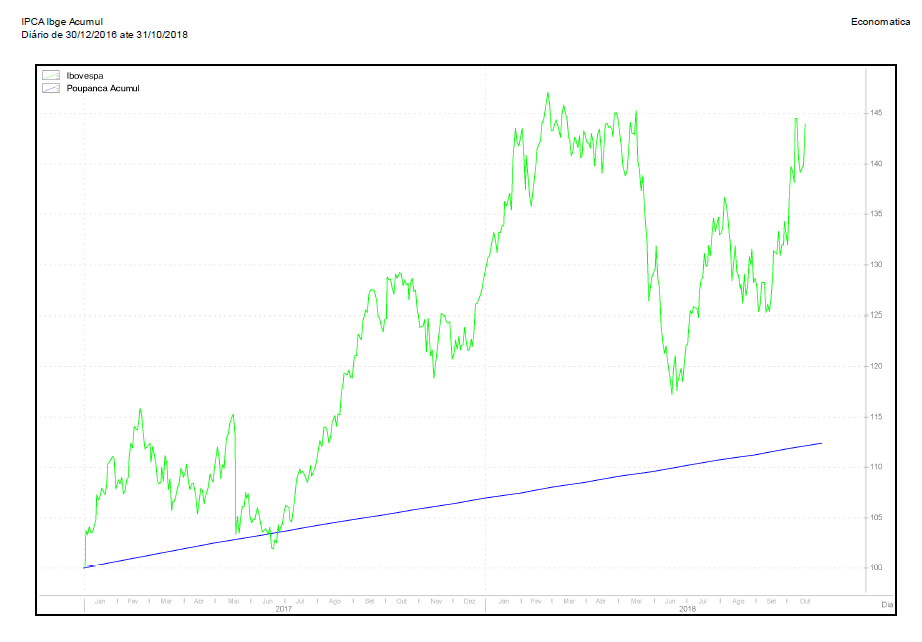
\includegraphics[width=1\linewidth]{figure/poupanca-ou-acoes-grafico} \caption{Uma comparação entre poupança vs. IBOV, de 2016 a 2018. Fonte: Econometrica}\label{fig:ibovpoupanca}
  \end{figure}
  Interessantemente, o único período no exposto acima que a poupança superou o IBOV foi nos momentos posteriores ao \emph{Joesley Day}, em 18 de maio de 2017.
  
  falar sobre democratizacao da bolsa (falar sobre bogle e etfs)
  
  Assim sendo, é importante de que as escolhas de ativos seja racional.
  falar sobre a importancia da racionalidade nas escolhas (procurar referencias)
  
  \hypertarget{objetivos}{%
  \section{Objetivos}\label{objetivos}}
  \begin{itemize}
  \tightlist
  \item
    fazer o valuation da COPEL via fluxo de caixa descontado e relativo
  \item
    fazer uma comparacao dos resultados
  \item
    alguma outra coisa
  \end{itemize}
  \hypertarget{limitauxe7uxf5es}{%
  \section{Limitações}\label{limitauxe7uxf5es}}
  
  \hypertarget{estrutura-do-trabalho}{%
  \section{Estrutura do trabalho}\label{estrutura-do-trabalho}}
  
  \hypertarget{o-mercado-de-energia}{%
  \chapter{O mercado de energia}\label{o-mercado-de-energia}}
  
  \hypertarget{agentes-regulatuxf3rios}{%
  \section{Agentes regulatórios}\label{agentes-regulatuxf3rios}}
  
  \hypertarget{mme}{%
  \subsection{MME}\label{mme}}
  
  \hypertarget{aneel}{%
  \subsection{ANEEL}\label{aneel}}
  
  \hypertarget{ons}{%
  \subsection{ONS}\label{ons}}
  
  \hypertarget{ccee}{%
  \subsection{CCEE}\label{ccee}}
  
  \hypertarget{epe}{%
  \subsection{EPE}\label{epe}}
  
  \hypertarget{o-fluxo-de-energia}{%
  \section{O fluxo de energia}\label{o-fluxo-de-energia}}
  
  \hypertarget{gerauxe7uxe3o}{%
  \subsection{Geração}\label{gerauxe7uxe3o}}
  
  \hypertarget{transmissuxe3o}{%
  \subsection{Transmissão}\label{transmissuxe3o}}
  
  \hypertarget{comercializauxe7uxe3o}{%
  \subsection{Comercialização}\label{comercializauxe7uxe3o}}
  
  \hypertarget{distribuiuxe7uxe3o}{%
  \subsection{Distribuição}\label{distribuiuxe7uxe3o}}
  
  \hypertarget{estudos-e-projeuxe7uxf5es-de-longo-prazo}{%
  \section{Estudos e projeções de longo prazo}\label{estudos-e-projeuxe7uxf5es-de-longo-prazo}}
  
  \hypertarget{plano-decenal-de-expansuxe3o-de-energia-pde}{%
  \subsection{Plano Decenal de Expansão de Energia (PDE)}\label{plano-decenal-de-expansuxe3o-de-energia-pde}}
  
  \hypertarget{plano-nacional-de-energia-pne}{%
  \subsection{Plano Nacional de Energia (PNE)}\label{plano-nacional-de-energia-pne}}
  
  \hypertarget{referencial-teuxf3rico}{%
  \chapter{Referencial teórico}\label{referencial-teuxf3rico}}
  
  \hypertarget{demonstrauxe7uxf5es-financeiras}{%
  \section{Demonstrações financeiras}\label{demonstrauxe7uxf5es-financeiras}}
  
  \hypertarget{demonstrativo-de-resultados-do-exercuxedcio-dre}{%
  \subsection{Demonstrativo de Resultados do Exercício (DRE)}\label{demonstrativo-de-resultados-do-exercuxedcio-dre}}
  
  \hypertarget{balanuxe7o-patrimonial-bp}{%
  \subsection{Balanço Patrimonial (BP)}\label{balanuxe7o-patrimonial-bp}}
  
  \hypertarget{demonstrativo-de-fluxo-de-caixa-dfc}{%
  \subsection{Demonstrativo de Fluxo de Caixa (DFC)}\label{demonstrativo-de-fluxo-de-caixa-dfc}}
  
  \hypertarget{valuation-intruxednseco}{%
  \section{\texorpdfstring{\emph{Valuation} intrínseco}{Valuation intrínseco}}\label{valuation-intruxednseco}}
  
  \hypertarget{muxe9todo-do-fluxo-de-caixa-descontado}{%
  \subsection{Método do Fluxo de Caixa Descontado}\label{muxe9todo-do-fluxo-de-caixa-descontado}}
  
  \hypertarget{valuation-relativo}{%
  \section{\texorpdfstring{\emph{Valuation} relativo}{Valuation relativo}}\label{valuation-relativo}}
  
  \hypertarget{anuxe1lise-por-muxfaltiplos}{%
  \subsection{Análise por múltiplos}\label{anuxe1lise-por-muxfaltiplos}}
  
  \hypertarget{estudo-de-caso}{%
  \chapter{Estudo de caso}\label{estudo-de-caso}}
  
  \hypertarget{contextualizauxe7uxe3o-da-copel}{%
  \section{Contextualização da COPEL}\label{contextualizauxe7uxe3o-da-copel}}
  
  \hypertarget{histuxf3ria}{%
  \subsection{História}\label{histuxf3ria}}
  
  \hypertarget{core-business}{%
  \subsection{\texorpdfstring{\emph{Core business}}{Core business}}\label{core-business}}
  
  \hypertarget{gerauxe7uxe3o-1}{%
  \subsubsection{Geração}\label{gerauxe7uxe3o-1}}
  
  \hypertarget{transmissuxe3o-1}{%
  \subsubsection{Transmissão}\label{transmissuxe3o-1}}
  
  \hypertarget{distribuiuxe7uxe3o-1}{%
  \subsubsection{Distribuição}\label{distribuiuxe7uxe3o-1}}
  
  \hypertarget{outros}{%
  \subsubsection{Outros}\label{outros}}
  
  \hypertarget{cuxe1lculo-do-valuation-intruxednseco}{%
  \section{\texorpdfstring{Cálculo do \emph{valuation} intrínseco}{Cálculo do valuation intrínseco}}\label{cuxe1lculo-do-valuation-intruxednseco}}
  
  \hypertarget{o-custo-de-capital-muxe9dio-ponderado-wacc}{%
  \subsection{O custo de capital médio ponderado (WACC)}\label{o-custo-de-capital-muxe9dio-ponderado-wacc}}
  
  \hypertarget{custo-de-capital-pruxf3prio}{%
  \subsubsection{Custo de capital próprio}\label{custo-de-capital-pruxf3prio}}
  
  \hypertarget{custo-de-capital-de-terceiros}{%
  \subsubsection{Custo de capital de terceiros}\label{custo-de-capital-de-terceiros}}
  
  \hypertarget{fluxo-de-caixa-descontado}{%
  \subsubsection{Fluxo de caixa descontado}\label{fluxo-de-caixa-descontado}}
  
  \hypertarget{cuxe1lculo-do-valuation-relativo}{%
  \section{\texorpdfstring{Cálculo do \emph{valuation} relativo}{Cálculo do valuation relativo}}\label{cuxe1lculo-do-valuation-relativo}}
  
  \hypertarget{margem-bruta}{%
  \subsection{Margem bruta}\label{margem-bruta}}
  
  \hypertarget{lucros-antes-de-juros-e-impostos-ebit}{%
  \subsection{Lucros antes de juros e impostos (EBIT)}\label{lucros-antes-de-juros-e-impostos-ebit}}
  
  \hypertarget{margem-luxedquida}{%
  \subsection{Margem líquida}\label{margem-luxedquida}}
  
  \hypertarget{razuxe3o-preuxe7olucro-pe}{%
  \subsection{Razão preço/lucro (P/E)}\label{razuxe3o-preuxe7olucro-pe}}
  
  \hypertarget{retorno-sobre-patrimuxf4nio-luxedquido-roe}{%
  \subsection{Retorno sobre patrimônio líquido (ROE)}\label{retorno-sobre-patrimuxf4nio-luxedquido-roe}}
  
  \hypertarget{comparauxe7uxe3o-com-empresas-do-setor}{%
  \subsection{Comparação com empresas do setor}\label{comparauxe7uxe3o-com-empresas-do-setor}}
  
  \hypertarget{conclusuxe3o}{%
  \chapter{Conclusão}\label{conclusuxe3o}}
  
  \backmatter
  
  \hypertarget{referuxeancias-bibliogruxe1ficas}{%
  \chapter*{Referências Bibliográficas}\label{referuxeancias-bibliogruxe1ficas}}
  \addcontentsline{toc}{chapter}{Referências Bibliográficas}
  
  \markboth{References}{References}
  
  \label{bib:begin}
  \noindent
  
  \setlength{\parindent}{-0.20in}
  \setlength{\leftskip}{0.20in}
  \setlength{\parskip}{8pt}
  
  \hypertarget{refs}{}
  \leavevmode\hypertarget{ref-bogle2015}{}%
  BOGLE, J. C. \textbf{Bogle on mutual funds: New perspectives for the intelligent investor}. Tradução:. New Jersey, John Wiley \& Sons, 2015.
  
  \leavevmode\hypertarget{ref-techreport-exampleIn}{}%
  GARRET, D. A. \textbf{The Microscopic Detection of Corrosion in Aluminum Aircraft Structures with Thermal Neutron Beams and Film Imaging Methods}. In: Report, nº NBSIR 78-1434. Washington, D.C., National Bureau of Standards, 1977.
  
  \leavevmode\hypertarget{ref-article-example}{}%
  IESAN, D. "Existence Theorems in the Theory of Mixtures", \textbf{Journal of Elasticity}, v. 42, n. 2, p. 145--163, fev. 1996..
  
  \leavevmode\hypertarget{ref-markowitz1952}{}%
  MARKOWITZ, H. "Portfolio selection", \textbf{The Journal of Finance}, v. 7, n. 1, p. 77--91, 1952..
  
  \leavevmode\hypertarget{ref-valorinveste2020}{}%
  NEIRA, A. C., FILGUEIRAS, I. \textbf{Número de pessoas físicas na B3 tem alta recorde e bate 2.24 milhões em março}.. {[}S.l.{]}, Valor Investe. Disponível em: \url{https://valorinveste.globo.com/objetivo/hora-de-investir/noticia/2020/04/03/numero-de-pessoas-fisicas-na-b3-tem-alta-recorde-e-bate-224-milhoes-em-marco.ghtml}., abr. 2020

  \backmatter
  \bibliographystyle{coppe-unsrt}
  \bibliography{thesis}

  %\appendix
  %\include{appenA}
\end{document}
